So for the business process, as stated previously, we have a set of activities that organizes the trucks and their drivers.
In the goal of have them work rather optimally in an automated fashion.

And it goes as follows:

\begin{center}
    \includegraphics[width=0.8\textwidth]{images/flowchart}
\end{center}

As seen in the diagram, it is rather a simple flowchart, but that would require to have a lot real time data put in place,
to have it coordinate with the trucks and drivers, without any downtimes.
And to adapt to the needs in hand, they've put in place the following IT infrastructure:

\begin{center}
    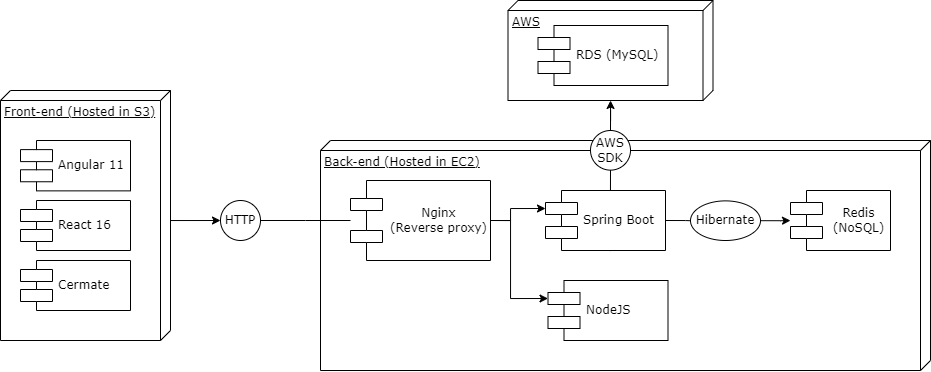
\includegraphics[width=0.8\textwidth]{images/State-of-art}
\end{center}

There are a lot of things that can be done to improve the performance of the system, but the main thing is to have a
base for the proof of concept.
As such, the released IT infrastructure is a good starting point for the proof of concept.